\chapter{Valg af hardware}

\section{Drone}

Det mest essentielle del til projektet er dronen. Derfor beskrives analyse og overvejelser lavet i forbindelse med dronens indkøb som det første.
  
Dronen til projektet blev valgt ud fra følgende punkter:
\begin{itemize}
	\item Pris.
	\item Løftekapacitet. 
	\item Tilgængelighed af reservedele. 
	\item Open source kode til regulering (motorstyring).
\end{itemize}

\vspace{0.5cm}

Ud fra kriterierne stod valget af drone mellem to forskellige quadrocopterer: 

\textbf{3DR} – Quadrocopter:  Det amerikanske firma 3D Robotics udvikler droner i forskellige størrelser. Quadrocopterer fra 3DR kan enten købes færdige eller som ”byg selv” projekter. Den bedst egnede quadrocopter fra 3DR er et ”byg selv” kit der hedder DIY Quad Kit\footnote{https://store.3drobotics.com/products/diy-quad-kit}. Ved køb af kittet fås 4x 10 x 4.7 propeller, 20 amp ESC’er og motorer der maksimalt yder 850 Kv.  Desuden medfølger et motorstyringsboard og styringssoftwaren er open source. Den samlede pris for DIY Quad kittet ligger på 549 USD. Det bemærkes, at batteri til quadrocopteren skal købes separat.

\textbf{AeroQuad}: Det Amerikanske firma AeroQuad har lavet quadrocopteren AeroQuad Cyclone ARF. Aeroquad'en\footnote{http://www.aeroquadstore.com/AeroQuad\textunderscore Cyclone\textunderscore ARF\textunderscore Kit\textunderscore p/aqarf-001.htm} er en lidt større quadrocopter med 12” propeller og motorer der yder 950 Kv ( 950 rpm/V). Til motorstyring følger open source styringssoftware samt fire 20 amp ESC'er med. Ydermere følger også tre pull og tre push propeller med. \newline Ligesom det var tilfældet 3DR, skal batteri til AeroQuad også købes separat. Ønskes yderligere reservedele, kan de købes via AeruoQuad’s hjemmeside. Prisen for en AeroQaud ligger på 509\$.

\newpage

Opsummering af de vigtigste funktionaliteterne i de to quadrocopterer:
\begin{table}[H]
	\centering
		\begin{tabular}{|p{3.5cm}|p{5 cm}|p{5 cm}|} 
		\hline
			\textbf{Specifikationer} & \textbf{3DR} 	& \textbf{Aeroquad} \\ \hline
					ESC'er &  4x med en maksimal belastning på 20 ampere				& 4x med en maksimal belastning på 20 ampere.	\\ \hline
			 		Motorer	& 4x 850 kV, børsteløse	& 4x 950 kV, børsteløse			\\ \hline
			 		Styringsboard	& 168MHz 32 bit ARM processor				& 168MHz 32 bit ARM processor		\\ \hline
			 			Propellere & 4x 10x4.7 			& 4x 12x2.8					\\ \hline
			 			Pris & 	550 \$	& 509 \$				\\ \hline
		\end{tabular}
	\caption{Opsummering}
	%\label{tab:TC1}
\end{table}

\vspace{1cm}

\begin{figure}[H]
\centering
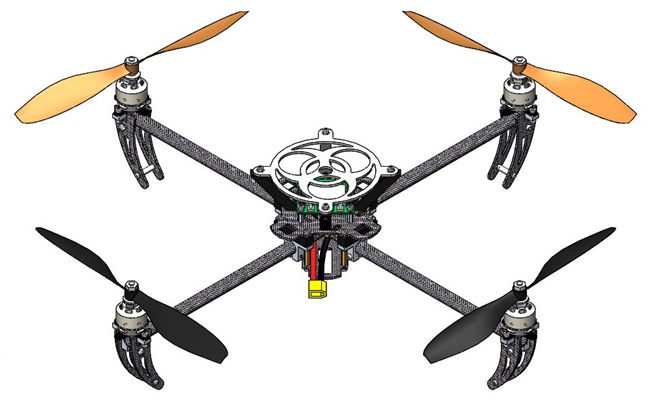
\includegraphics[width=0.7\textwidth]{Billeder/drone.png}
\caption{Aeroquad ARF}
\label{fig:Aeroquad ARF}
\end{figure}

\vspace{1cm}


Ud fra den overstående undersøgelse, ses det at Aeroquaden er lidt billigere end 3DR quadrocopter. Desuden har Aeroquad'en et større vingefang og motorer med højere rotationshastighed. Hvilket er faktorer der øger quadrocopterens løfteevne og stabilitet. Derfor blev Aeroquad's quadrocopter valgt til projektet.

